\chapter{Results and Discussion}

%%%%%%%%%%%%%%%%%%%%%%%%%%%%%%%%%%%%%%%
%%%%%%%%%%%%%%%%%%%%%%%%%%%%%%%%%%%%%%%
\section{Validation Tests}
The thermal wall plate is validated for three test cases: nominal ZPG turbulent boundary layer flow (1) over an isothermal wall plate, (2) encountering a sharp step in wall temperature, and (3) around a wall mounted hemisphere body. 
Wall-normal profiles of temperature and velocity across  the boundary layer are acquired for case (1) and (2). 
For case (3), IR imaging is used to show that the wall plate can maintain a constant temperature even when the flow above the wall is unsteady and strongly three-dimensional. 

\begin{figure}[h!]
  \begin{center}
  {\subfigcapskip = 5pt \subfigcapmargin = -12pt \subfigure[]{\label{fig:edge-a}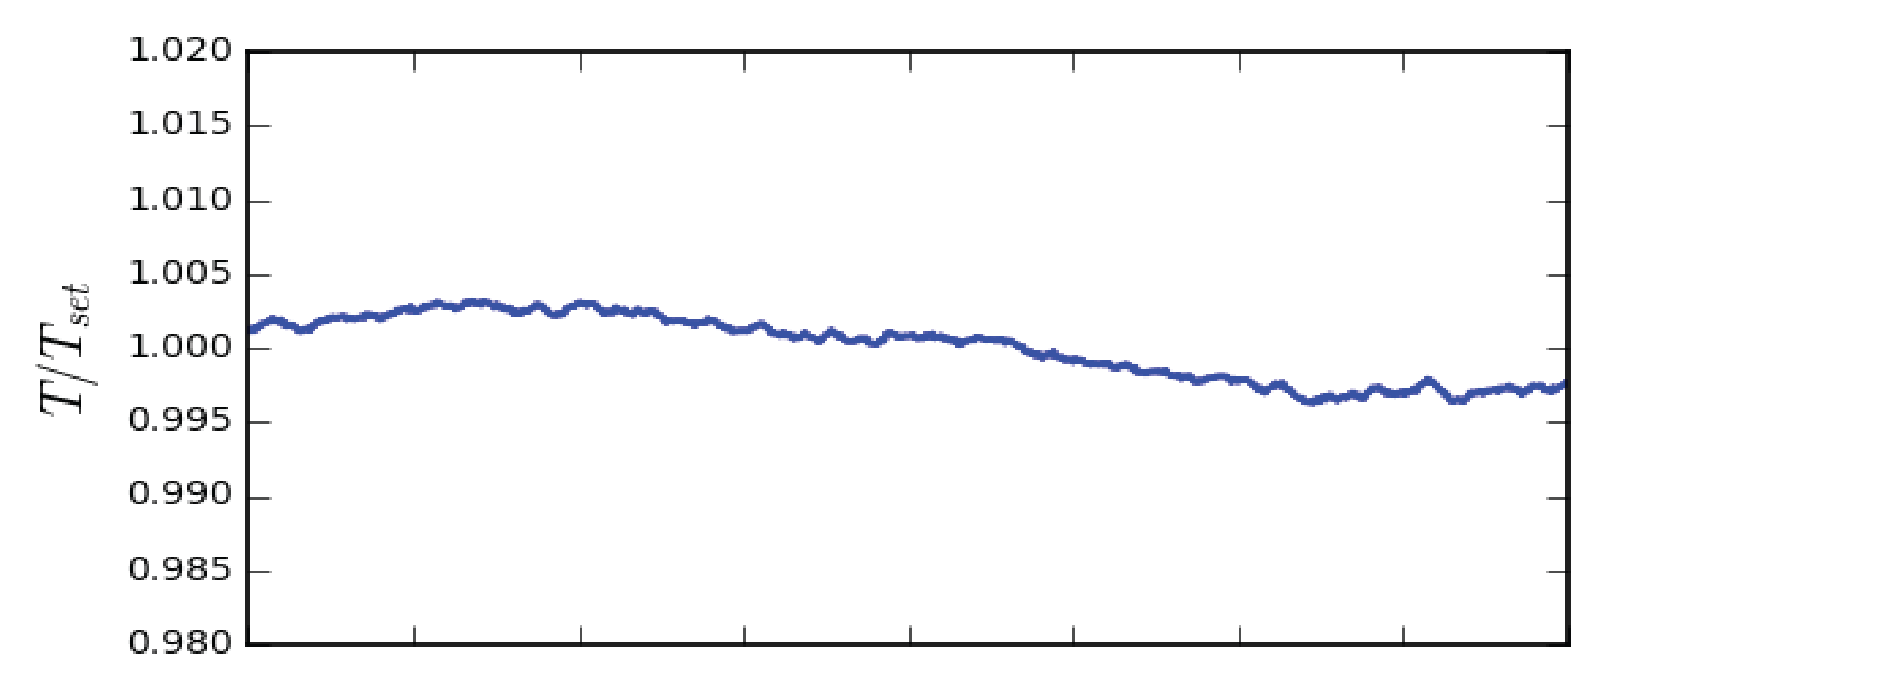
\includegraphics[scale=0.5]{results/IR_distribution_V5_a.png}}}
   {\subfigcapskip = 5pt \subfigcapmargin = -12pt  \subfigure[]{\label{fig:edge-b}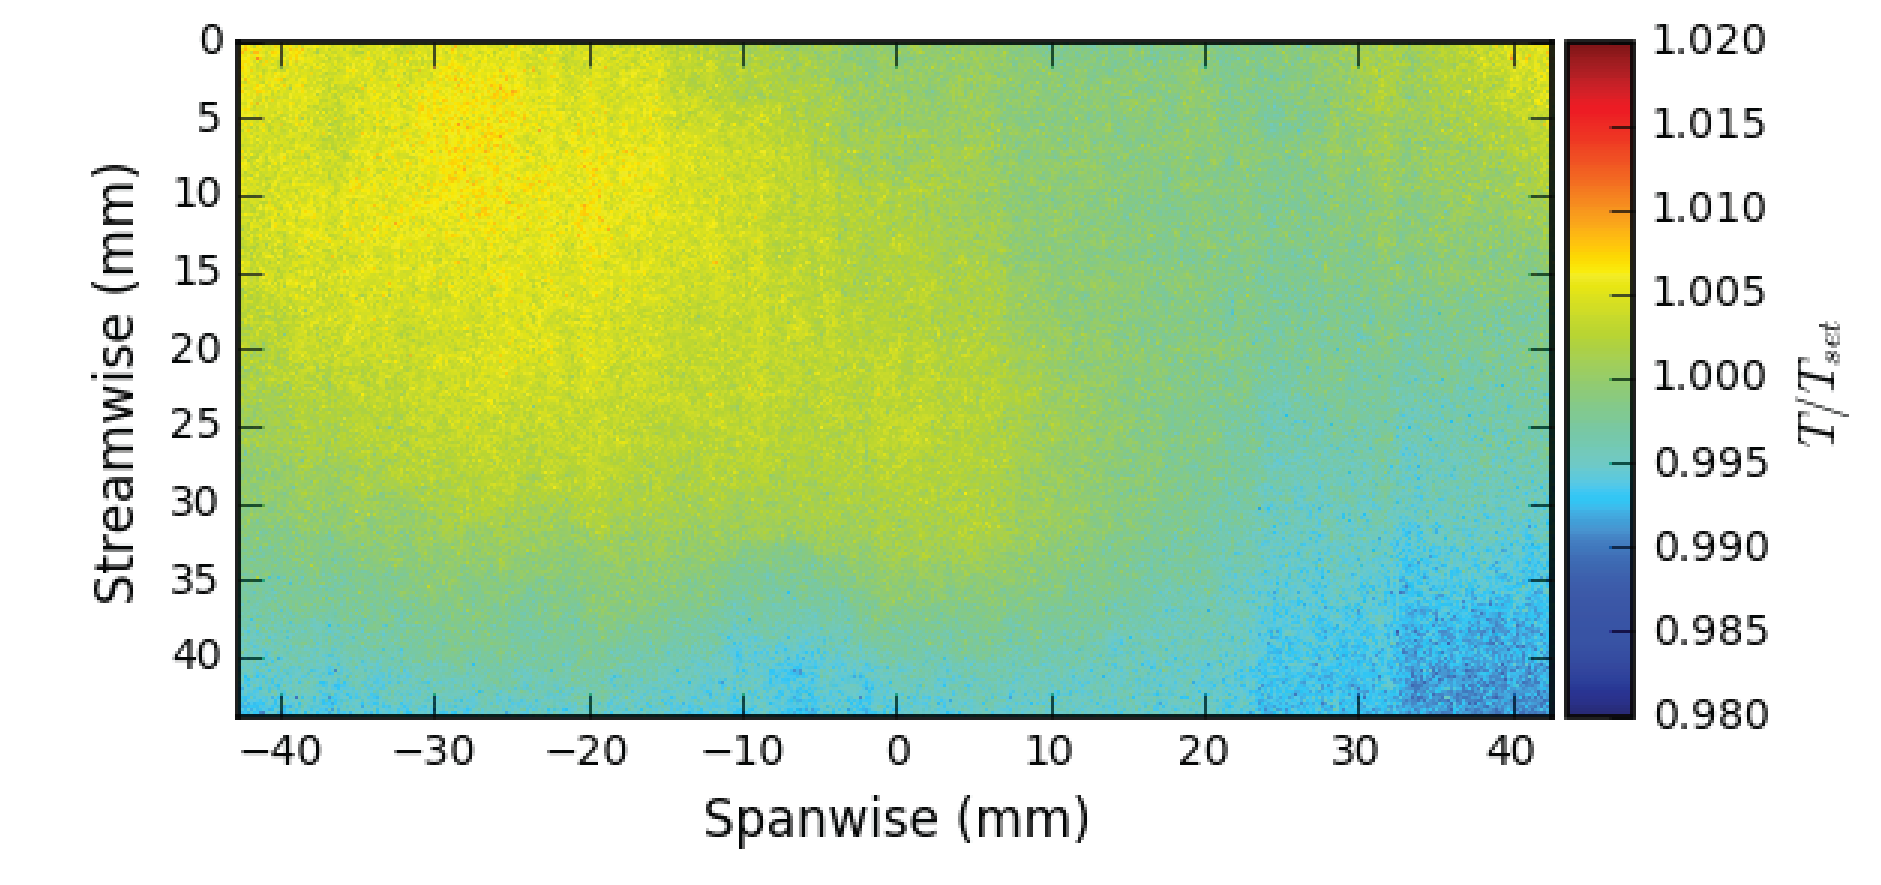
\includegraphics[scale=0.5]{results/IR_distribution_V5_b.png}}}
  \end{center}
\caption{(a) Representative ensemble-averaged IR image of plate \#5 for $T_{set} = 40^\circ$C. (b) Spanwise profile of streamwise averaged temperature from figure (a).} 
\label{fig:IR-ZPG}
\end{figure}


%%%%%%%%%%%%%%%%%%%%%%%%%%%%%%%%%%%%%%%%%%%%%%%%
\subsection{ZPG turbulent boundary layer flow over an isothermal wall plate}
The freestream temperature  of the air in the tunnel is set to 25$^\circ$C and each section of the thermal wall plate is set to 40$^\circ$C.
Measurements are acquired at five different momentum thickness Reynolds numbers, $Re_\theta$, as listed in Table~\ref{tab:temp}. 
The freestream velocity is steady with magnitudes varying between 2--10 ms$^{-1}$. 
The FLIR SC645 IR camera is positioned above plate \#5 located 0.8m downstream of the trip and the FOV is 85mm $\times$ 64mm in the spanwise and streamwise directions, respectively. 
The temperature of the convective plate was evaluated by ensemble-averaging 100 IR images acquired at 16Hz to reduce pixel-noise. 
The effect of averaging over shorter or longer periods showed no statistical difference between the results.

Fig.~\ref{fig:IR-ZPG}(a) shows a representative ensembled-averaged IR image of the thermal wall plate. 
The colorbar represents $T/T_{set}$ where $T_{set}$ is 40$^\circ$C.
The range of the color bar magnitude is $\pm$ 5\% of the set-point temperature. Spatially averaging the corresponding image in the streamwise direction results in the averaged spanwise temperature profile shown in Fig.~\ref{fig:IR-ZPG}(b). 
Note that the spanwise variation is less than the measurement uncertainty of the IR temperature measurement which is $\pm 2\% \approx \pm 0.8 ^\circ$C.  
In brief, the IR images show that the thermal wall plate can be held to a constant temperature within a tolerance that is less than the measurement uncertainty of the camera. 
The embedded thermocouples, located just downstream of Fig.~\ref{fig:IR-ZPG}(a) and at spanwise locations of 0 and $\pm$ $75mm$, indicate the spanwise gradient to be much smaller and that the tolerance of the wall plate temperature is $\pm 0.5^\circ$C.

\begin{figure}[h!]
  \begin{center}
  {\subfigcapskip = 5pt \subfigcapmargin = -12pt \subfigure[]{\label{fig:edge-a}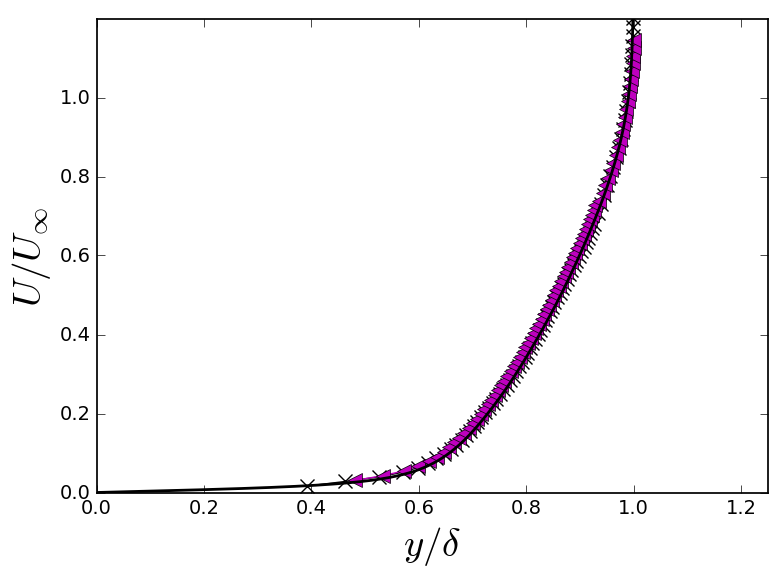
\includegraphics[scale=0.36]{results/heat_noheat_outer.png}}}
   {\subfigcapskip = 5pt \subfigcapmargin = -12pt  \subfigure[]{\label{fig:edge-b}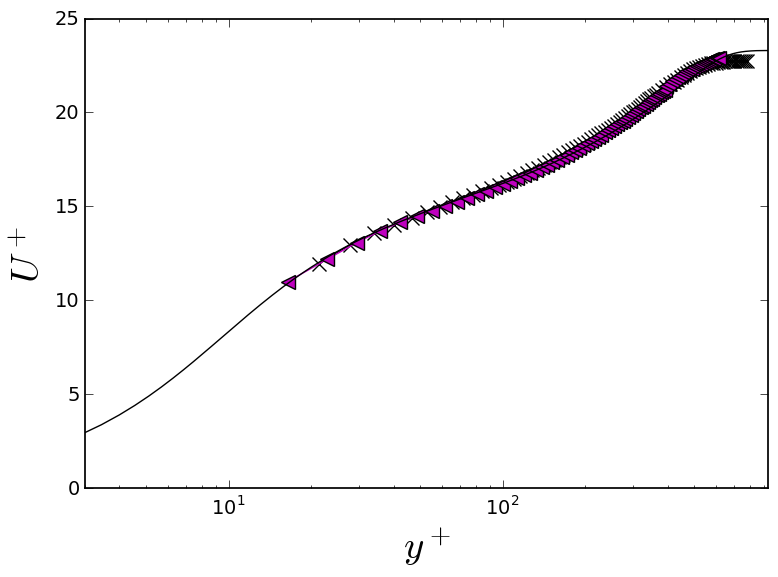
\includegraphics[scale=0.36]{results/heat_noheat_inner.png}}}
  \end{center}
 \caption{Wall-normal profiles of mean streamwise velocity at $Re_\theta=1527$ with thermal wall plate on ($\times$)  and off ($\triangleleft$) plotted in (a) outer-coordinates and (b) inner-coordinates. The solid lines denote the data from \cite{Wu2010} at a similar $Re$.}
\label{fig:ZPG-velocity}
\end{figure}

It is first shown that the momentum boundary layer behaves as expected, through the agreement with the DNS data, and the collapse of the two mean velocity profiles demonstrates that temperature behaves like a passive scalar. 
The wall-normal mean velocity profile was obtained by ensemble-averaging over 30,000 instantaneous PIV vector fields and then spatially averaging over the streamwise ($x-$) direction. 
The corresponding mean velocity profiles from camera 1 and camera 2 were then stitched together following the method of Shea \textit{et al.} \cite{Shea2014} to obtain a profile that spans the entire wall-normal height of the boundary layer. 
The outer normalized mean velocity profiles when the thermal plate was at 40$^\circ$C and when the thermal plate was unheated is shown in Fig.~\ref{fig:ZPG-velocity}(a) (all other conditions being the same), where $U_\infty$ and $\delta$ are the freestream velocity and momentum boundary layer thickness, respectively. 
The same profiles plotted in so-called inner coordinates are shown  in Fig.~\ref{fig:ZPG-velocity}(b) (see Eq.~\ref{eq:lawofwall}). 
Here the wall shear stress was computed from the PIV data using the integral method of Mehdi $\textit{et. al}$ \cite{Mehdi2011}.  
The agreement with the DNS data and the apparent logarithmic region of the velocity profile demonstrates the flow over the plate is consistent with a canonical ZPG boundary layer.


\begin{table}[h]
\caption{Parameters for measured temperature profiles}
\centering
%\resizebox{\columnwidth}{!}{%
\begin{tabular}{|c|c|c|c|c|c|}
\hline 
Symbol & $T_{w} (^\circ C)$ & $U_{\infty} (ms^{-1})$ & $Re_{\theta}$ & $\delta_T (mm)$ & $u_\tau (ms^{-1})$\\ 
\hline 
\color{red}$\blacksquare$ & 40 & 1.95 & 568 & 38 & 0.10\\ 
\hline 
{\color{blue} x} & 40 & 2.87 & 825 & 34 & 0.14\\ 
\hline 
{\color{green} $\blacklozenge$} & 40 & 3.90 & 1147 & 34 & 0.17\\
\hline
{\color{magenta} $\blacktriangleleft$} & 40 & 5.04 & 1454 & 33 & 0.22\\
\hline
{\color{cyan} $\bullet$} & 40 & 9.15 & 2415 & 29 & 0.37\\
\hline
\end{tabular}%
%}
\label{tab:temp}
\end{table}

The wall-normal mean temperature profile was obtained by time averaging the thermocouple signal at a given $y$-position over a 100 seconds record length. 
Fig.~\ref{fig:ZPG-temp}(a) and Fig.~\ref{fig:ZPG-temp}(b) show the mean temperature profiles plotted in outer and inner-coordinates, respectively at five different values of $Re_\theta$ as described in Table~\ref{tab:temp} . 

Collectively, the two plots demonstrate that the measured temperature profile is consistent with a ZPG boundary layer over an isothermal wall with heat transfer.  

\begin{figure}[t!]
  \begin{center}
  {\subfigcapskip = 5pt \subfigcapmargin = -12pt \subfigure[]{\label{fig:edge-a}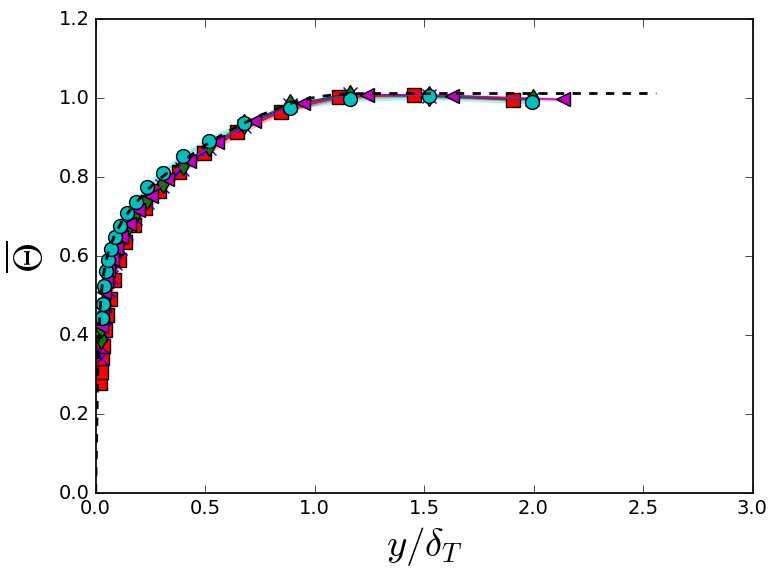
\includegraphics[scale=0.37]{results/theta_vs_yoverdeltaT.png}}}
   {\subfigcapskip = 5pt \subfigcapmargin = -12pt  \subfigure[]{\label{fig:edge-b}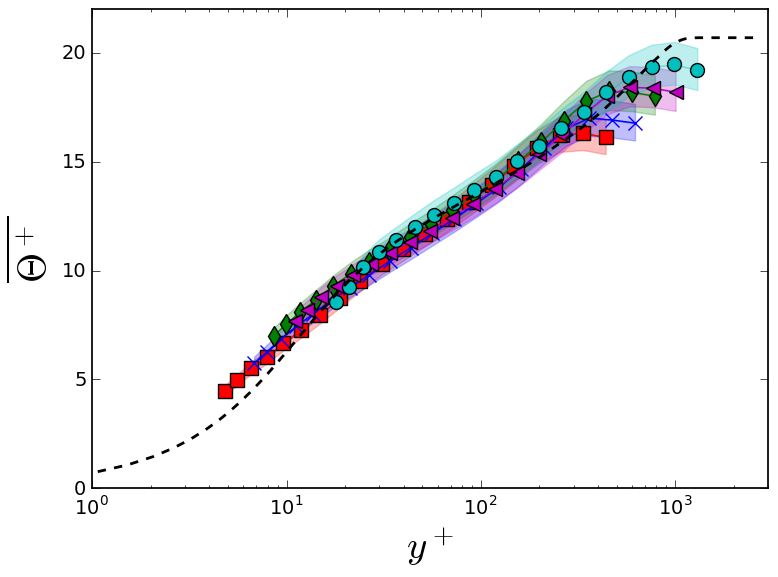
\includegraphics[scale=0.37]{results/thetaplus_vs_yplus_log.png}}}
  \end{center}
 \caption{Wall-normal profiles of mean temperature plotted in (a) outer-coordinates and (b) inner-coordinates. Shading denotes a $\pm 5\%$ variance in computed $u_\tau$ value. The dotted line denote the data from  Arya \textit{et al.} \cite{Araya2012} at $Re_\theta=2290$.}

\label{fig:ZPG-temp}
\end{figure}

%%%%%%%%%%%%%%%%%%%%%%%%%%%%%%%%%%%%%%
\subsection{ZPG boundary layer encountering a sharp step in wall temperature}
\begin{figure*}[h!]
\centering
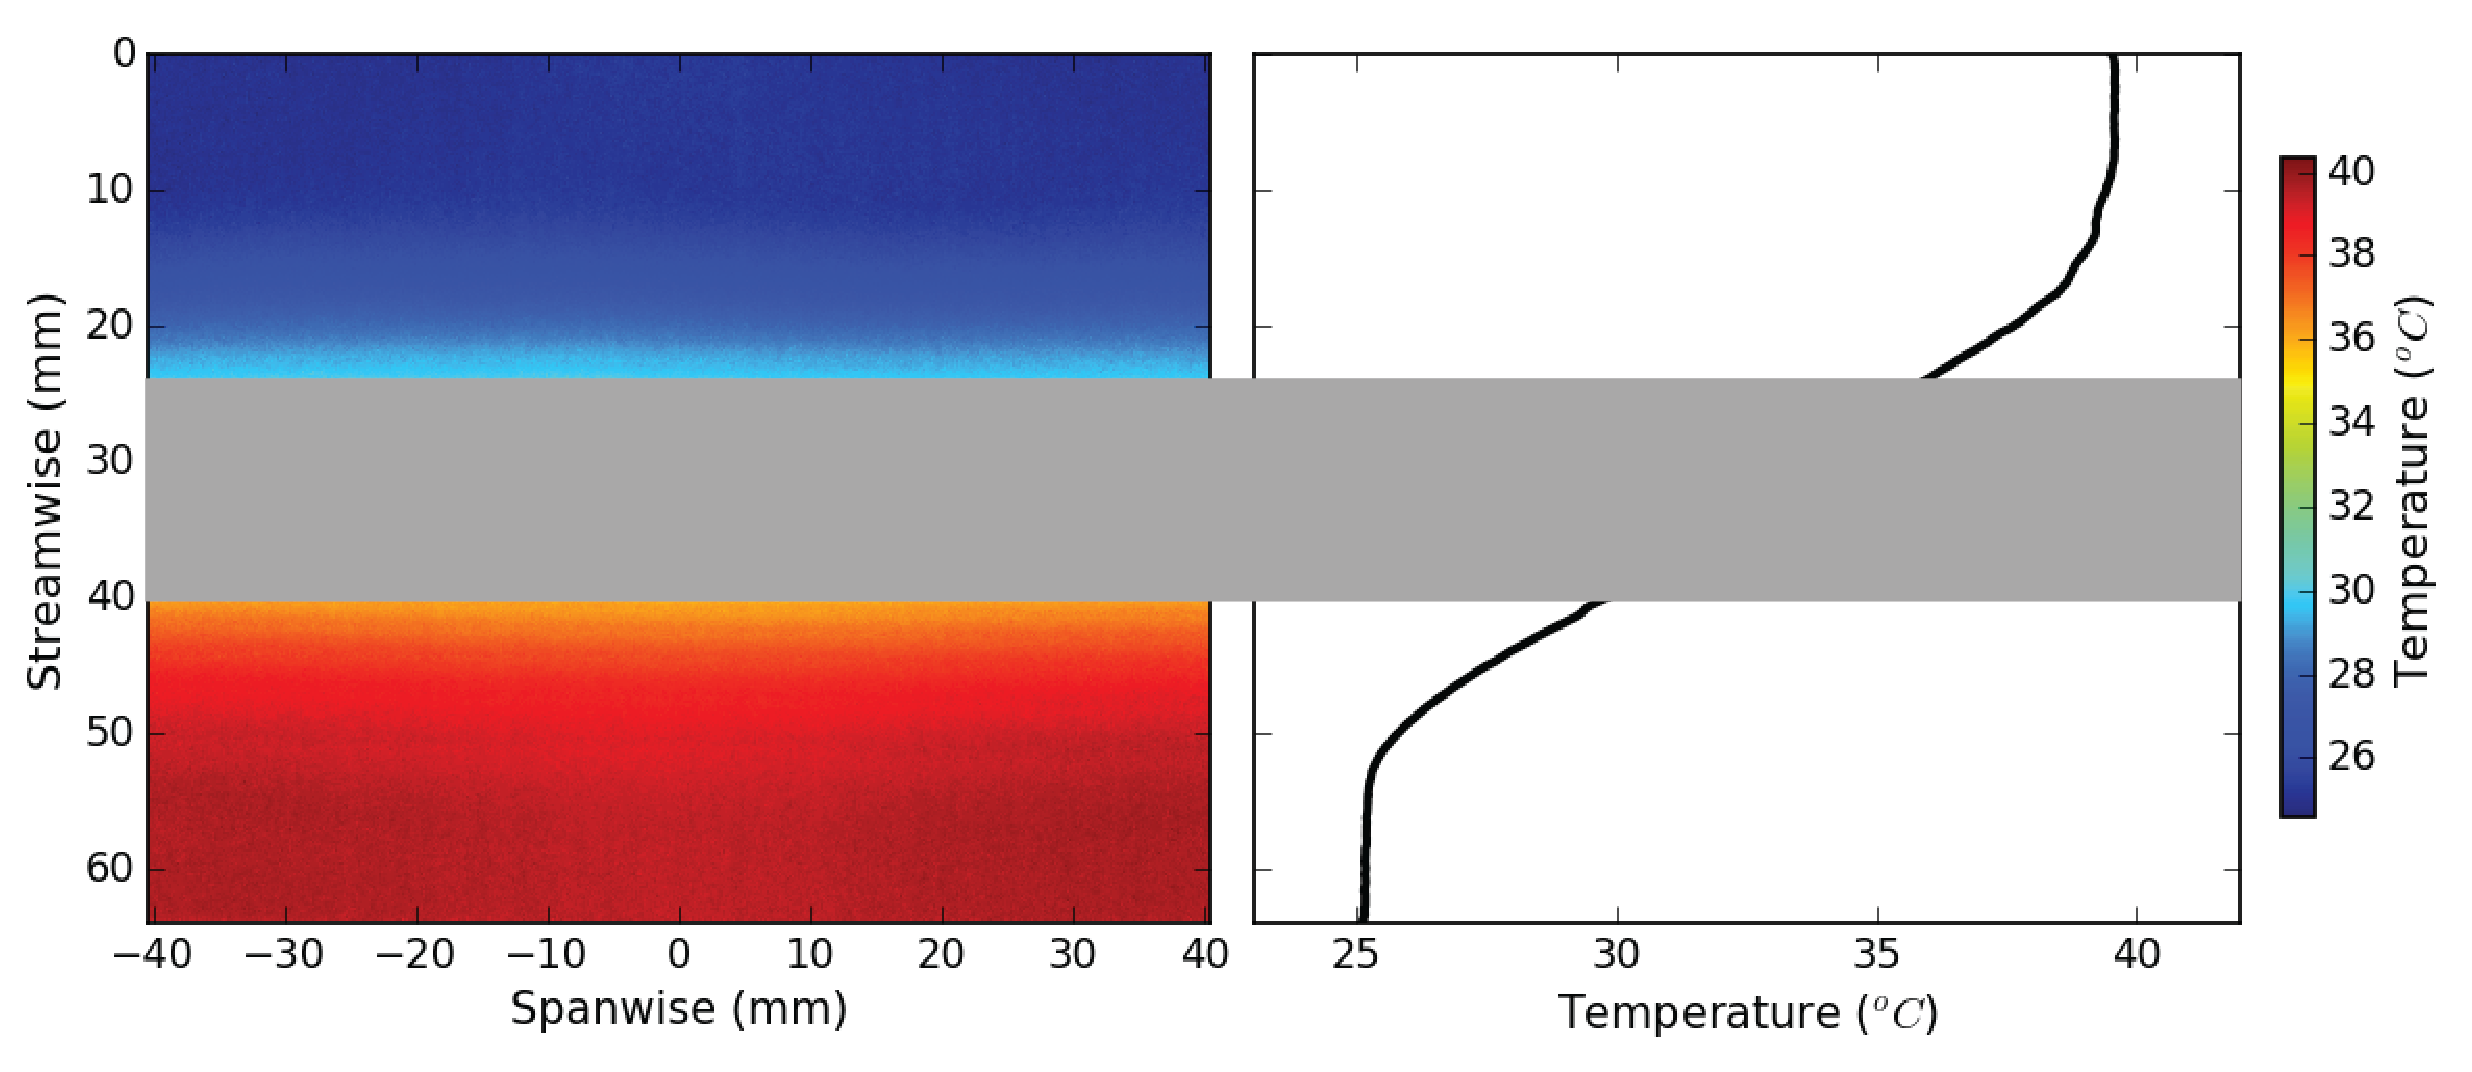
\includegraphics[scale=.5]{results/therm_step_IR_v6.png}
\caption{(a) Representative ensemble-averaged IR image of temperature step. The top-plate is unheated where T=$25^\circ$C and the bottom plate is set to T=40$^\circ$C. The flow is from top-to-bottom. (b) The streamwise profile of spanwise averaged temperature.} 
\label{fig:IR-STEP}
\end{figure*}

In this configuration, a ZPG turbulent boundary layer initially develops over an unheated portion of the wall-plate and then encounters a sharp one-dimensional step in wall temperature at some distance $x_T$ downstream of the boundary layer trip. 
Effectively, a thermal boundary develops internal to an existing turbulent momentum boundary layer. 
The configuration is relevant to a flow where a boundary layer encounters a change in surface conditions such as when the atmospheric boundary layer flows from sea to land or when the flow over an engineered surface flows from a cold region to a hot region.  
Owing to its importance in both geophysical flows and engineering systems, this particular flow configuration has been fairly well-studied in the literature \cite{Antonia1977,Hoffmann1979, Moretti1965} and is therefore an appropriate test case for validating the NEAT boundary layer facility. 

In the present study, the length of the unheated portion of the wall plate is varied by systematically changing the start location of the temperature step relative to the trip position. 
A sting-mounted type J fine-wire ($0.65mm$ probe diameter) thermocouple attached to a Velmex BiSlide traverse was placed $1.26m$ downstream of the trip (i.e., in the middle of plate $\#$9). 
The freestream velocity was set to $4ms^{-1}$ and wall-normal temperature profiles were acquired for varying unheated starting lengths. 
The temperature of the convective plate where the temperature step occurred and those downstream of the step were set to $40^\circ$C while the convective plates upstream of the step were unheated. 
In terms of the convective plate numbers, the first profile was acquired when only plate \#9 was heated, the second profile was acquired when plates \#8 and \#9 were heated and so forth until the last profile was acquired when plates \#1-9 were heated.  
Note that in this configuration, the thickness of the momentum boundary layer within which the thermal boundary layer begins to grow varies from profile to profile. 

Fig.~\ref{fig:IR-STEP}(a) shows a representative ensembled-averaged IR image of the temperature step. 
The flow is from top-to-bottom and the colorbar represents the surface temperature of the plate. The top-plate is unheated where $T=25^\circ$C and the bottom plate is set to $T=40^\circ$C.  
Fig.~\ref{fig:IR-STEP}(b) shows the mean streamwise temperature profile obtained by spatially averaging in the spanwise direction. 
The thermal jump is considered a sharp thermal interface with a thermal gradient of 450$^\circ$C per meter ($0.45^\circ$C/mm), which is greater than that investigated by Moretti $\textit{ et al.}$ \cite{Moretti1965}. 
Note that the temperature of the insulating region separating the plates cannot be accurately determined from the IR images owing to the difference in emissivity between the insulated region and the convective plate. 
The embedded thermocouples show the temperature difference between the two plates to be 15 $^\circ$C.  

\begin{figure}[h]
  \begin{center}
  {\subfigcapskip = 5pt \subfigcapmargin = -12pt \subfigure[]{\label{fig:edge-a}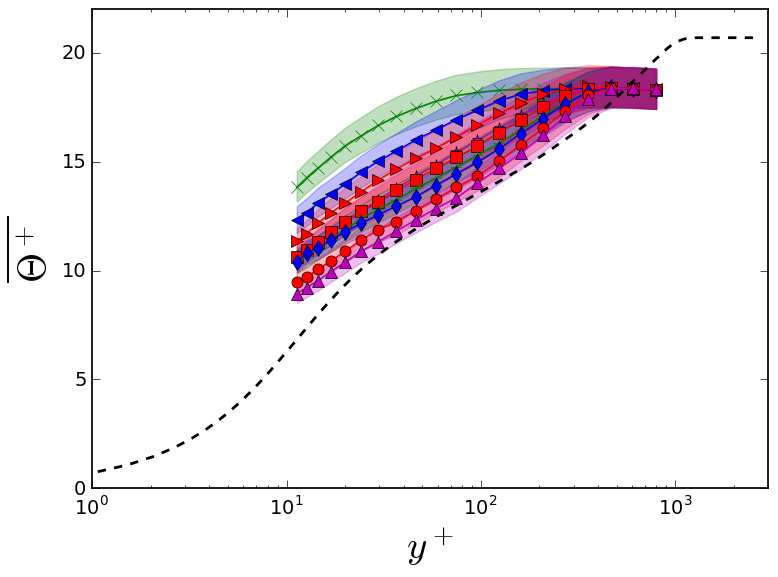
\includegraphics[scale=0.32]{facility/therm_step_inner_log.png}}}
   {\subfigcapskip = 5pt \subfigcapmargin = -12pt  \subfigure[]{\label{fig:edge-b}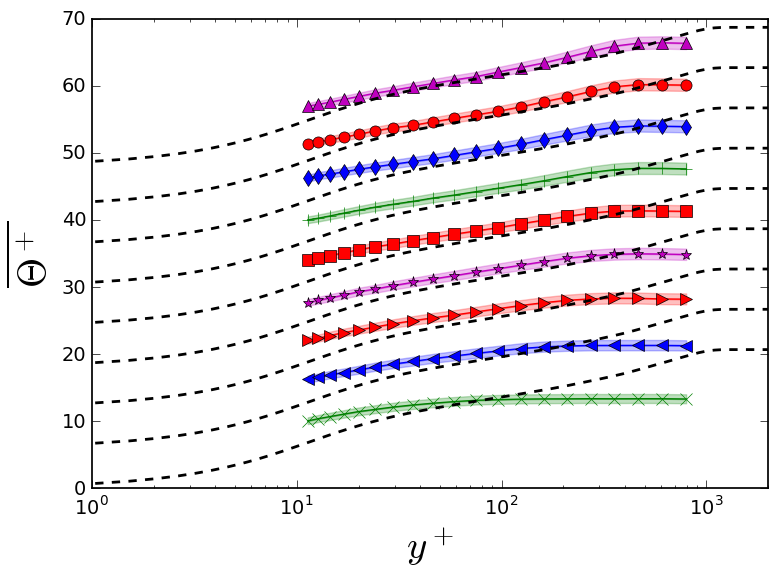
\includegraphics[scale=0.32]{facility/therm_step_inner_log_offset.png}}}
  \end{center}
 \caption{Wall-normal profiles of mean temperature after thermal step. Plates heated corresponding to profiles is as follows; $\#$9 {\color{green} $\times$}, $\#$8-9 {\color{blue} $\blacktriangleleft$}, $\#$7-9 {\color{red} $\blacktriangleright$}, $\#$6-9 {\color{purple} $\bigstar$}, $\#$5-9 {\color{red} $\blacksquare$}, $\#$4-9 {\color{green} $+$}, $\#$3-9 {\color{blue} $\blacklozenge$}, $\#$2-9 {\color{red} $\bullet$}, $\#$1-9 {\color{purple} $\blacktriangle$}. Plotted in (a) inner-coordinates using $St$ (Eq.~\ref{eq:qw}), and (b) modified inner-coordinates using $St_T$ (Eq.~\ref{eq:st_correction}), subsequent profiles are offset by $\Theta^+=6$ for visual clarity. The dotted line denotes the law of the wall turbulent profile.}
\label{fig:Step-temp}
\end{figure}


The wall-normal (y-direction) mean temperature profile was obtained by time averaging the thermocouple signal at a given $y$-position over a record length of 100 seconds ($\approx1000 \delta/u_\tau$).
Fig.~\ref{fig:Step-temp} shows the mean temperature profiles plotted in outer and inner coordinates for the nine different unheated starting lengths. 
Owing to the difficulty of evaluating $\delta_T$ for short thermal development lengths (i.e, large $x_T$ with fixed profile measurement location), the so-called thermal displacement thickness given by 

\begin{equation}
\delta_T^* = \int_0^\infty \frac{T(y) - T_\infty}{T_w - T_\infty} dy,
\end{equation}

\noindent was used for outer normalization \cite{Antonia1977}.  The wall heat flux values used for inner-normalization is determined from the correlation 

\begin{equation}
St(x) = St_T \left[ 1 - \left(\frac{x_T}{x}\right)^{9/10}\right]^{-1/9}
%St(x) = 0.0287 Re_x^{-0.2}Pr^{-0.4} \left[ 1 - \left(\frac{x_T}{x_o}\right)^{9/10}\right]^{-1/9}
\label{eq:st_correction}
\end{equation}

\noindent developed by \cite{Reynolds1958} as as an approximate solution for the heat transfer downstream of a wall temperature step in a ZPG boundary layer flow, where $St_T$ is given by Eq.~\ref{eq:qw} and $x_T$ is the unheated starting length. 
The profiles (each shifted by $\Theta^+ = 6$) show approximate collapse on the expected turbulent profile (dashed lines in the figure) that improves with decreasing $x_T$ . 
These datasets demonstrate that the flow over the plate encountering a wall temperature step is consistent with previous studies \cite{Reynolds1958, Hoffmann1979}, validating the ability of the thermal wall plate to produce temperature step wall boundary conditions.



%%%%%%%%%%%%%%%%%%%%%%%%%%%%%%%%%%%
\subsection{ZPG turbulent boundary layer flow around a wall mounted hemisphere body}

\begin{figure}[h!]
\centering
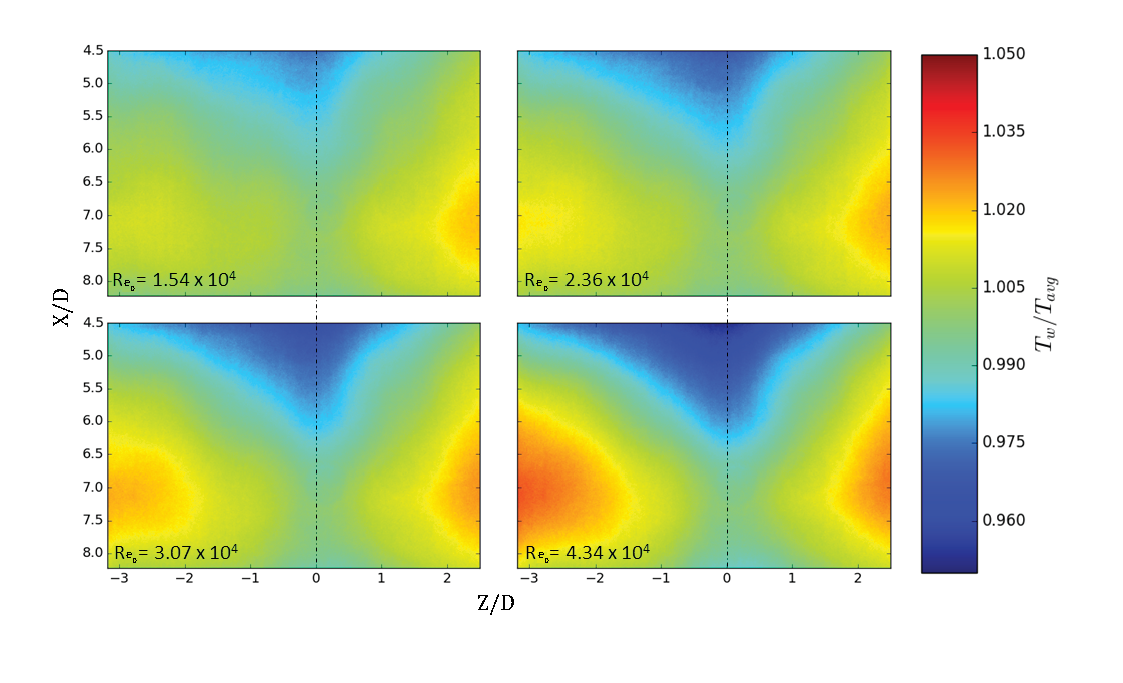
\includegraphics[scale=.75]{results/hemi_IR.eps}
\caption{Spatial temperature distributions located downstream of a hemisphere for four values of $Re_D$. The streamwise and spanwise positions have been normalized by the hemisphere diameter $D$ = 3cm.} 
\label{fig:IR-HEMI}
\end{figure}

When a boundary layer flow encounters a wall-mounted hemisphere body, the pressure gradients around the hemisphere lead to the formation of a necklace vortex at the hemisphere base with legs that extend downstream \cite{simpson2001}. 
Flow separation at the top of the hemisphere produces vortex loops in the near-wake region \cite{Savory1986,Hansen1975}.
The vorticity in far wake structure is comprised of both the necklace vortex and the vortex loops (see Fig.~\ref{fig:HEMI-Cartoon}). 
The influence of these types of fluid-structure interactions on heat transfer are important across a broad range of problems from flow over glaciers to atmospheric re-entry vehicles. 

In the present study, a wall mounted hemisphere body of diameter D = 3cm was placed on the leading edge nose just upstream of the first convective wall plate. 
The boundary layer upstream of the hemisphere is laminar and the boundary layer is thin compared to the hemisphere with $\delta/D \approx 0.1$.  
The set point temperature of the convective wall plate was 60$^\circ$C. The inlet air was unheated with $T_\infty = 23^\circ$C. 
IR images of the thermal wall plate were acquired downstream of the hemisphere with an imaged area from $4.5 \lessapprox X/D \lessapprox 8.2$ (i.e., near the trailing edge of the first conductive wall plate) and from $-3.0 \lessapprox Z/D \lessapprox 2.5$, where $Z/D=0$ denotes the centerline of the hemisphere in the streamwise direction. 
Ensemble-averaged IR images of the spatial distribution of the wall plate temperature at four values of $Re_D$ are shown in Fig.~\ref{fig:IR-HEMI}. 
The colormap corresponds to the plate temperature normalized by the average temperature of the plate.  

The spatial distribution of temperature in the IR images show a distinct pattern that becomes more pronounced with increasing $Re_D$. 
The spatial pattern of temperature indicates that wake vorticity carries cold freestream fluid towards the wall near the plane of symmetry (i.e. near $Z/D = 0$ in the figure). 
The tapered pattern of minimum temperature (maximum heat transfer) is consistent with the study of \cite{Chyu1996} where local mass (heat) transfer measurements were acquired using naphthalene sublimation that showed a similar tapered shape and that the maximum heat transfer occurred near the reattachment point (which is likely upstream the measurement field-of-view near $X/D \approx 2.5$.) 
The high temperature lopes in the pattern likely result from the spanwise motion of high temperature fluid along the wall (see Fig.~\ref{fig:HEMI-Cartoon} plane view). 
Moreover, the center of the lope is likely a signature of the vortex structure driving the spanwise motion. 

\begin{figure*}[h!]
\centering
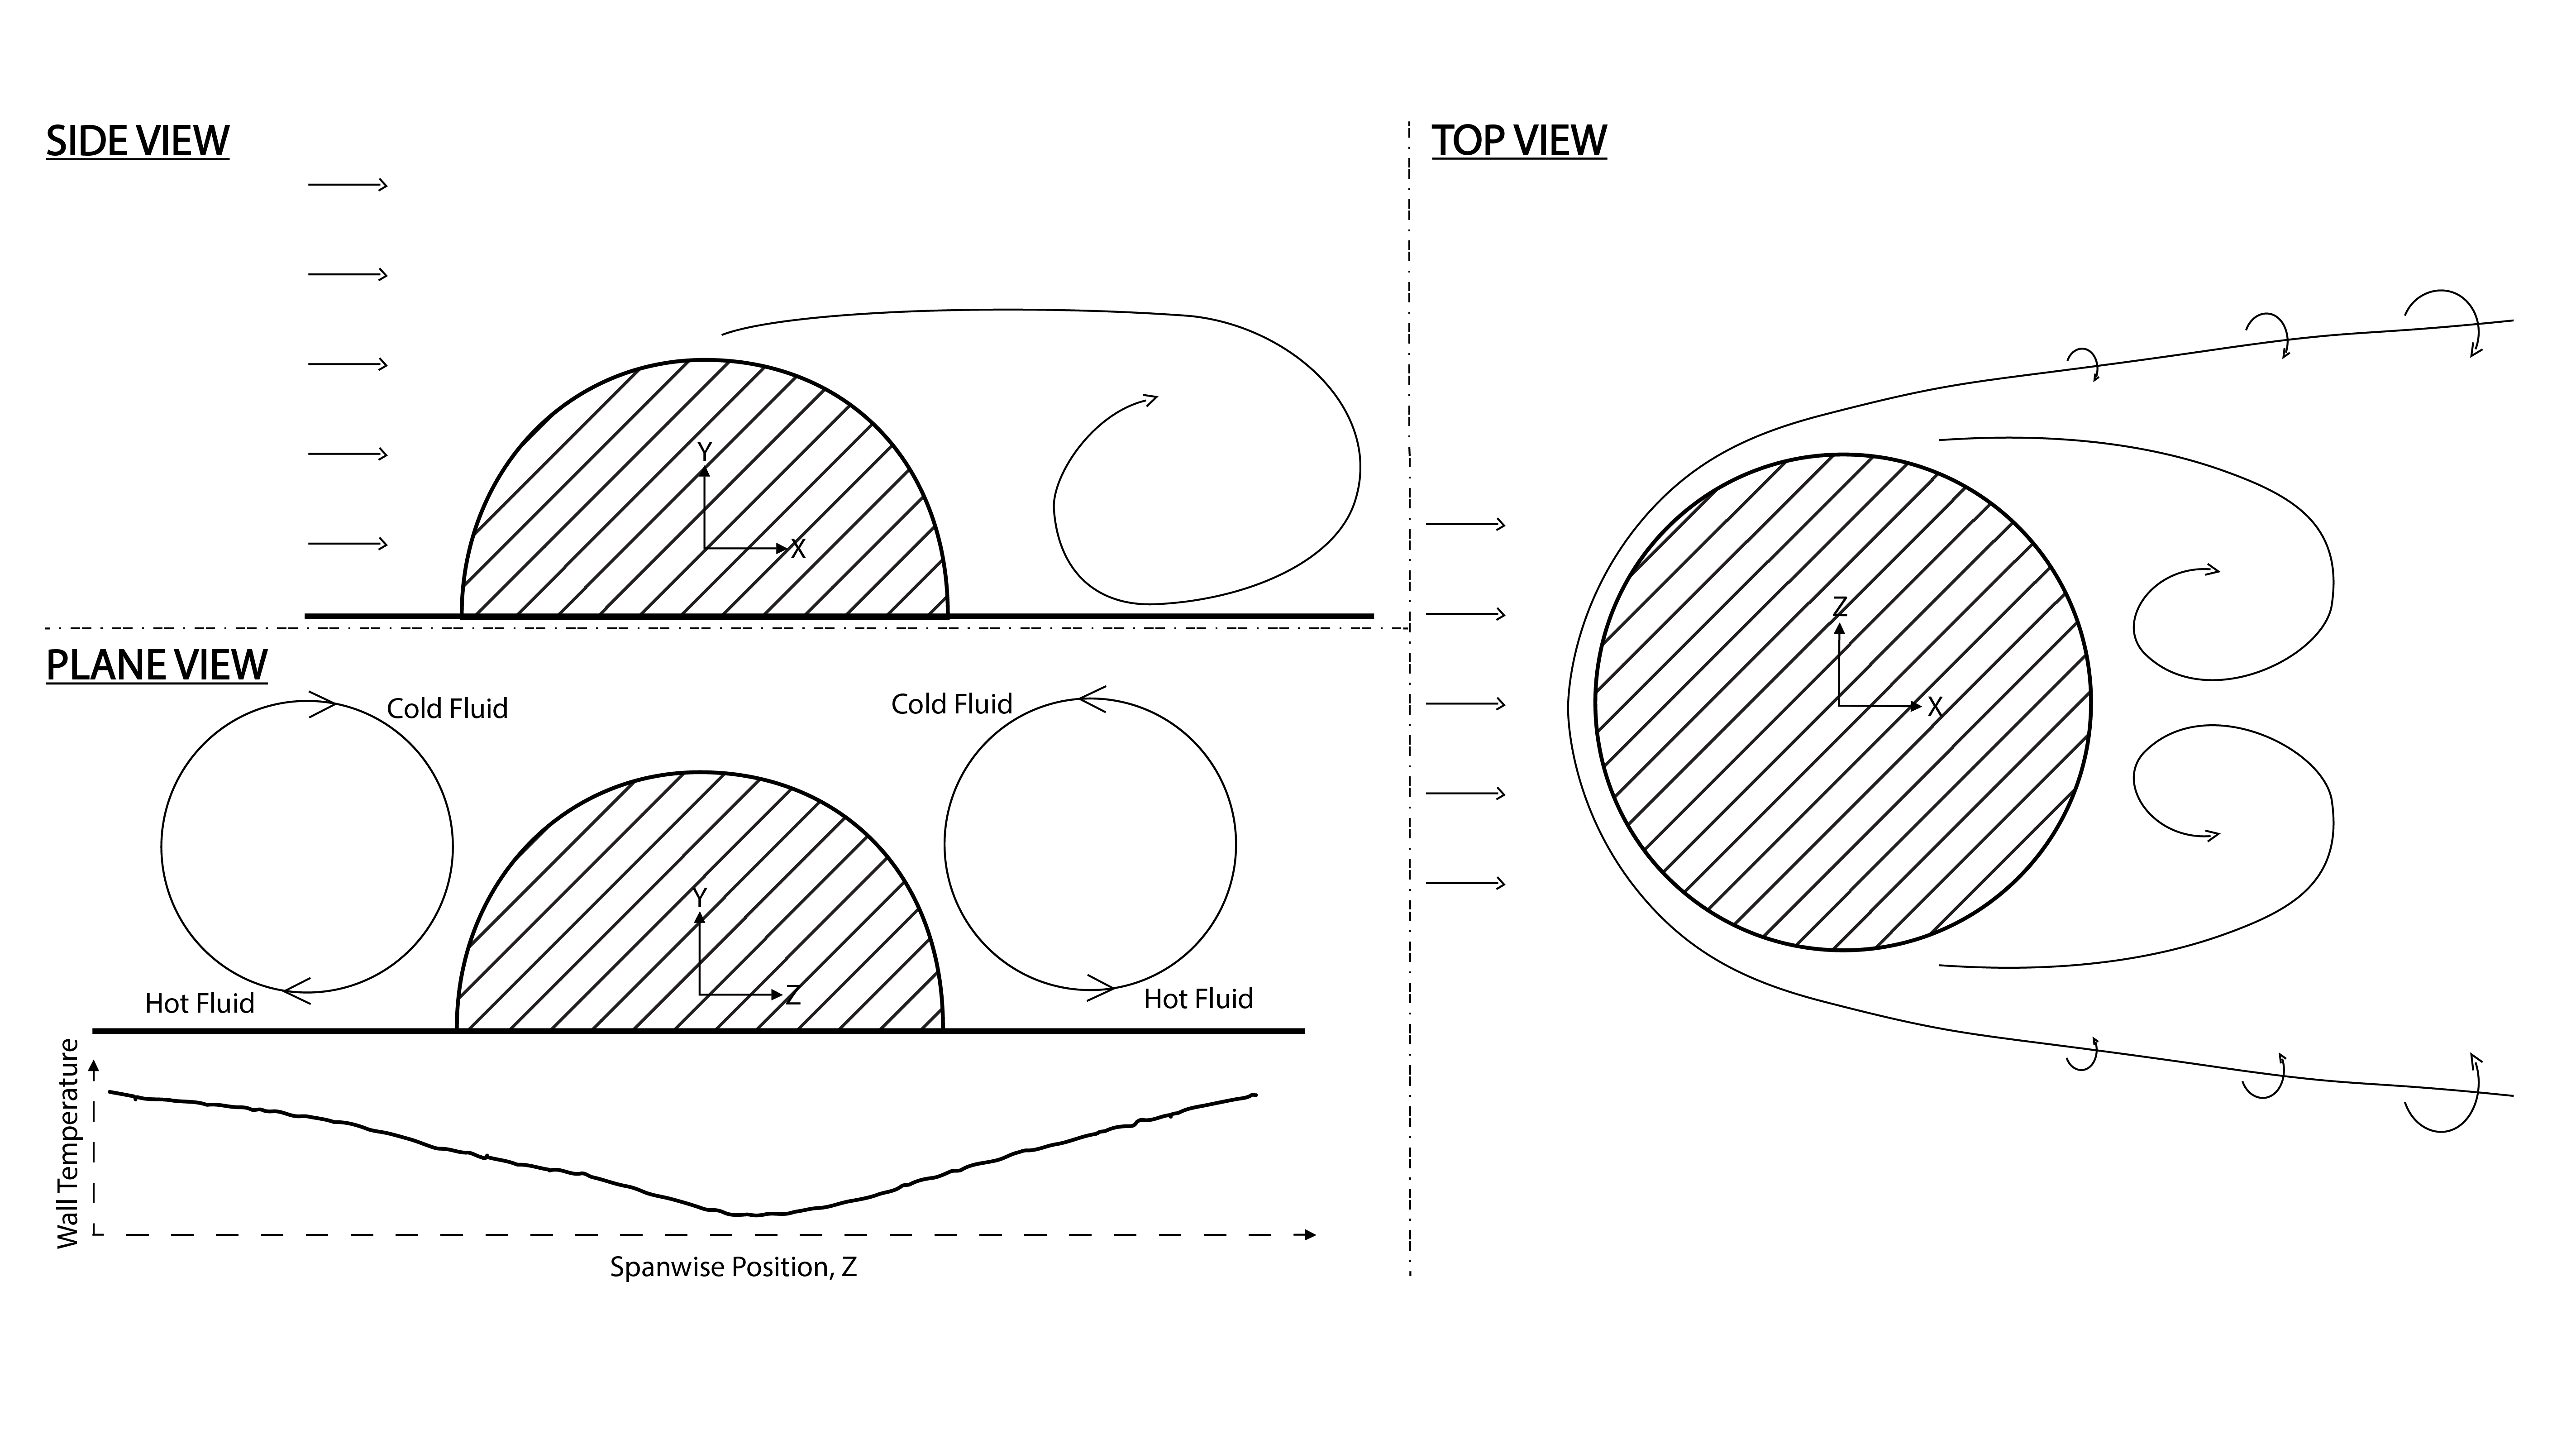
\includegraphics[scale=.3]{results/hemi_cartoon_v3.png}
\caption{Two plane view of cartoon depiction for resulting flow field from hemisphere perturbation. The XZ plane provides a birds eye view of the developing vortex wake, and the YZ plane provides a view of vortex wake downstream of the hemisphere and the resulting wall temperature.} 
\label{fig:HEMI-Cartoon}
\end{figure*}

While the pattern observed in Fig.~\ref{fig:IR-HEMI} is interesting and informative of the flow structure above the plate, it is evident that the wall-plate temperature is not constant as desired but varies by approximately $\pm$5\% across the convective plate. 
The difficulty of course is that large spatial variations in the convective heat transfer coefficient exist across the convective plate owing to the strong three dimensionality of the flow behind the hemisphere. 
Since the design purpose was to set and hold fixed the convective wall plate temperature at a desired temperature, the design needed to be modified. 
This was accomplished by first replacing each of the two center thin film resistive heaters by two heaters of half the original size, now giving 4 separate heaters in the middle section of the convective plate. 
Next, the number of controllers was increased from one to two, one for each half of the convective plate. 
Then the number of controllers was increased from two to three controllers, where the center controller was used for the center two resistive heaters and the remaining two controllers were used for the left and right section of the plate. 
The mean spanwise temperature profile obtained by spatially averaging in the streamwise direction is shown in Fig.~\ref{fig:hemi-control}  for each control scheme at $Re_D = 2.4 \times 10^4$. 

The profiles for two and three controllers shows that the spatial variation is further reduced by increasing the number of independent controllers. 
By using three controllers, the spatial variation of temperature is within $\pm$ 1\% which is less than the measurement uncertainty of the IR temperature measurement. 
Given this lack of resolution it is difficult to assess the apparent asymmetry in the profiles but a reasonable assumption is that the asymmetry is likely due to somewhat different responses of the left and right controller. 
In brief, these results demonstrate the ability of the thermal wall plate design to be easily adjusted to maintain a nearly uniform wall temperature in a highly three-dimensional flow.

\begin{figure}[h!]
\centering
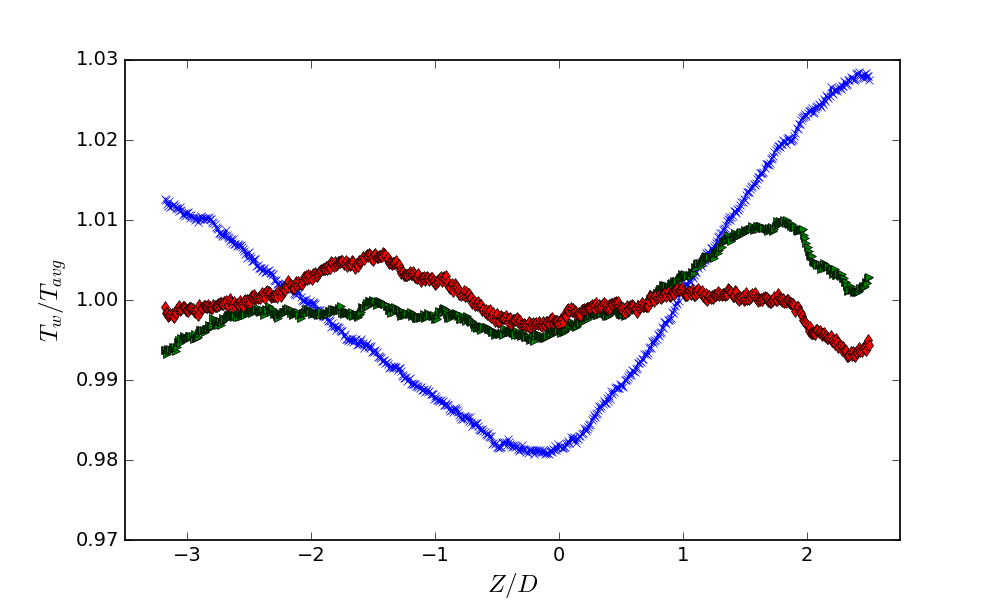
\includegraphics[width=\columnwidth]{results/hemi_multicontrollers_profile.png}
\caption{{\footnotesize Spanwise temperature profiles taken from the center of the IR images at a downstream position of 1 controller, {\color{blue}X};  2 controllers, {\color{green}$\blacktriangleright$}; 3 controllers, {\color{red}$\blacklozenge$}}}
\label{fig:hemi-control}
\end{figure}


%%%%%%%%%%%%%%%%%%%%%%%%%%%%%%%%%%%%%
%%%%%%%%%%%%%%%%%%%%%%%%%%%%%%%%%%%%%
\section{Non-equilibrium Flow}



%%%%%%%%%%%%%%%%%%%%%%%%%%%%%%%%%%%%%
%%%%%%%%%%%%%%%%%%%%%%%%%%%%%%%%%%%%%
\section{Modified Correlations}